\documentclass{beamer}
\usepackage[utf8]{inputenc}
\usepackage[T2A,T1]{fontenc}
\usepackage[english, russian]{babel}
\usetheme{Pittsburgh}

\selectlanguage{russian}
\newcommand{\define}[2]{{\bf #1} --- #2.\vspace{1em}}
\newcommand{\longdef}[1]{{\textbf{\underline{Опр:}} #1}}
%Add identation from the left side for theorema text
\newcommand{\theorema}[1]{{\textbf{\underline{Теор:}} #1}}
\newcommand{\set}[1]{{\lbrace #1 \rbrace}}

\title{Аутентифицированные режимы шифрования}
\institute{ВГУ}
\date{2014}
\begin{document}

\frame{\titlepage}

\begin{frame}
  \frametitle{Цель лекции}

  \begin{itemize}
    \item{Симметричное шифрование обеспечивает сокрытие содержания передаваемых
      данных от ``пассивного`` злоумышленника}
    \item{MAC обеспечивает целостность передаваемых данных и подтверждение авторства}
  \end{itemize}

  \vspace{8mm}
  Цель лекции: обеспечение конфиденциальности и целостности данных при наличии ``активного`` злоумышленника.
\end{frame}

\begin{frame}
  \frametitle{Пример атаки для несанкционированного доступа к данным}

  Протокол IPsec.

  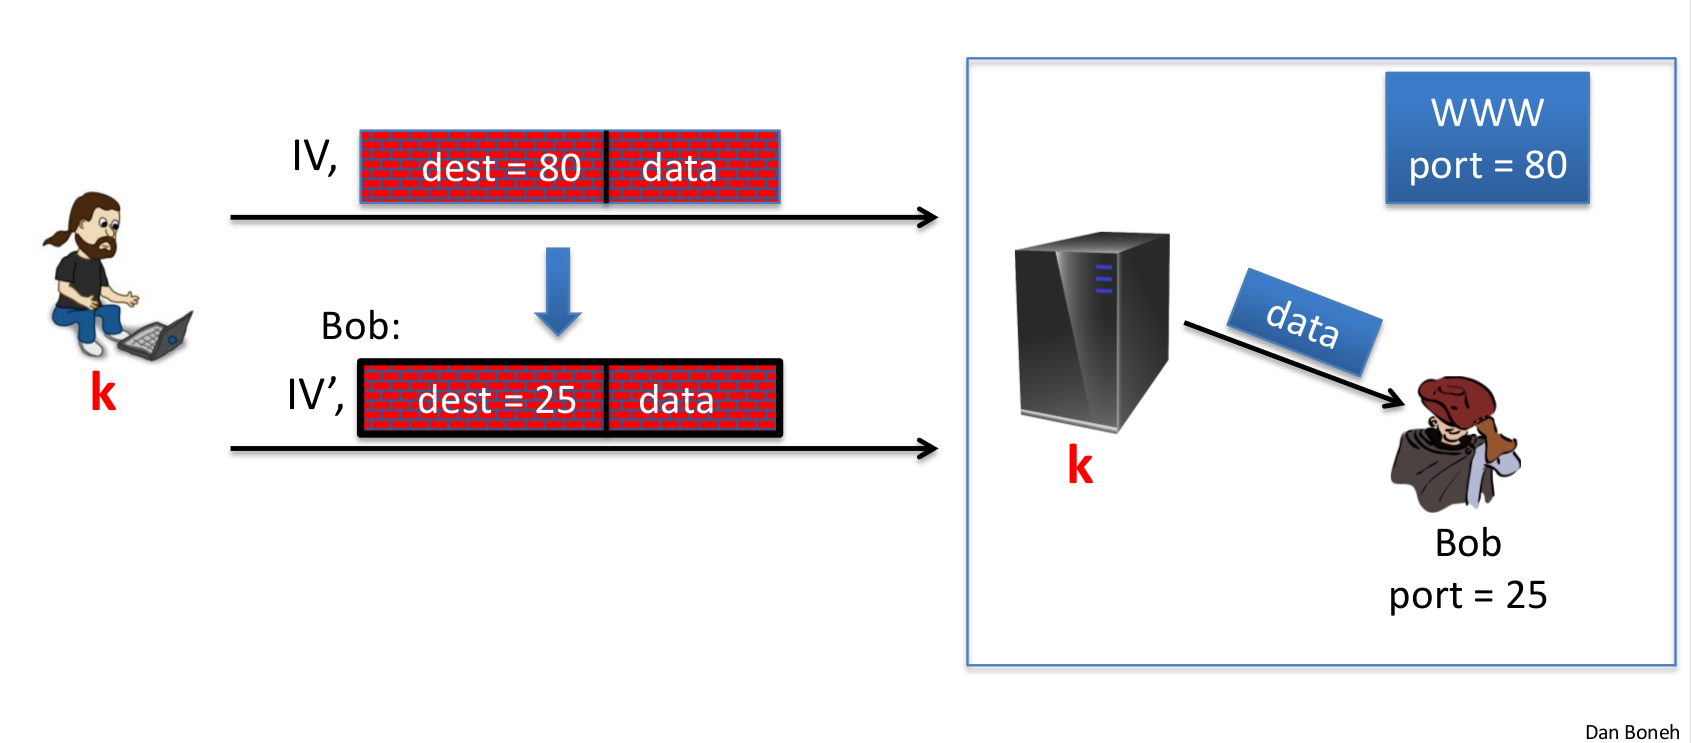
\includegraphics[width=\linewidth]{./img/png/ipsec_attack.png}

\end{frame}

\begin{frame}
  \frametitle{Выводы}

  Для защиты от ``активных`` злоумышленников необходимо применять:
  \begin{itemize}
    \item{\textbf{MAC}, если необходима целостность данных, но не конфиденциальность.}
    \item{\textbf{Аутентифицированные режимы шифрования}, если необходима как целостность данных,
      так и их конфиденциальность.}
  \end{itemize}
\end{frame}

\begin{frame}
  \frametitle{Определение}

  \textbf{Система с аутентифицированным режимом шифрования} это пара алгоритмов ($E$, $D$), где:
  \[ E: K \times M \rightarrow C \]
  \[ D: K \times C \rightarrow M \cup \{\bot\} \]

  Система должна обеспечивать:
  \begin{itemize}
    \item{Сокрытие данных от ``пассивных`` злоумышленников}
    \item{Целостность шифротекстов. Невозможно создать шифротекст $c$ без знания выбранного ключа $k$, чтобы $D(k, c) \neq \bot$}
  \end{itemize}
\end{frame}

\begin{frame}
  \frametitle{Свойства}

  Аутентификация сообщений

  \begin{itemize}
    \item{Злоумышленник не может обмануть Боба в том, что сообщение пришло от Алисы.}
    \item{Если при дешифровании $D(k, c) \neq \bot$ Боб может быть уверен, что
      сообщение пришло от того, кто знает секретный ключ (или сообщение является дубликатом одного из предыдущих)}
  \end{itemize}

  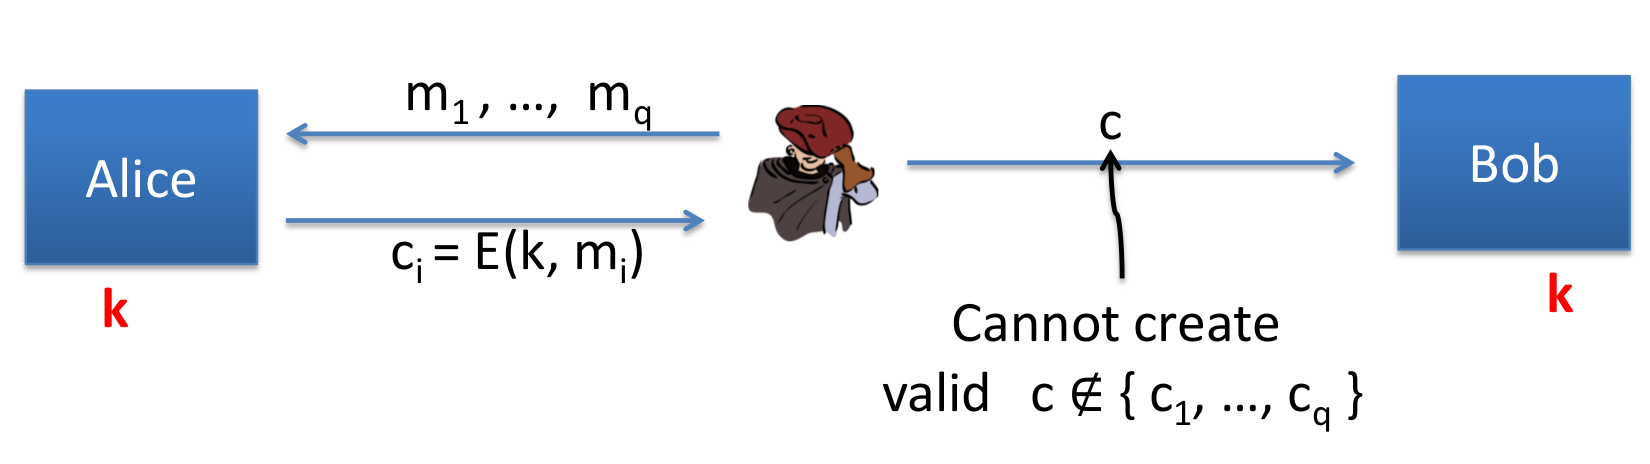
\includegraphics[width=\linewidth]{./img/png/authenticity.png}
\end{frame}

\begin{frame}
  \frametitle{Свойства}

  Защита от атак ``выбранного шифротекста``

  \begin{itemize}
    \item{Обеспечивает конфиденциальность от злоумышленника,
      который знает открытый текст для некоторых шифротекстов}
  \end{itemize}

\end{frame}

\begin{frame}
  \frametitle{История аутентифицированных режимов шифрования}

  \begin{itemize}
    \item{Понятие было введено в 2000 году}
    \item{До этого каждая криптографическая библиотека предоставляла отдельные API для симметричного шифрования и для MAC}
    \item{Пользователи библиотек должны были комбинировать вызовы для достижения аутентификации и конфиденциальности}
    \item{Иногда это приводило к небезопасным реализациям}
  \end{itemize}
\end{frame}

\begin{frame}
  \frametitle{Сочетание шифрования и МАС}

  Используются два ключа: ($k_{E}$, $k_{I}$)

  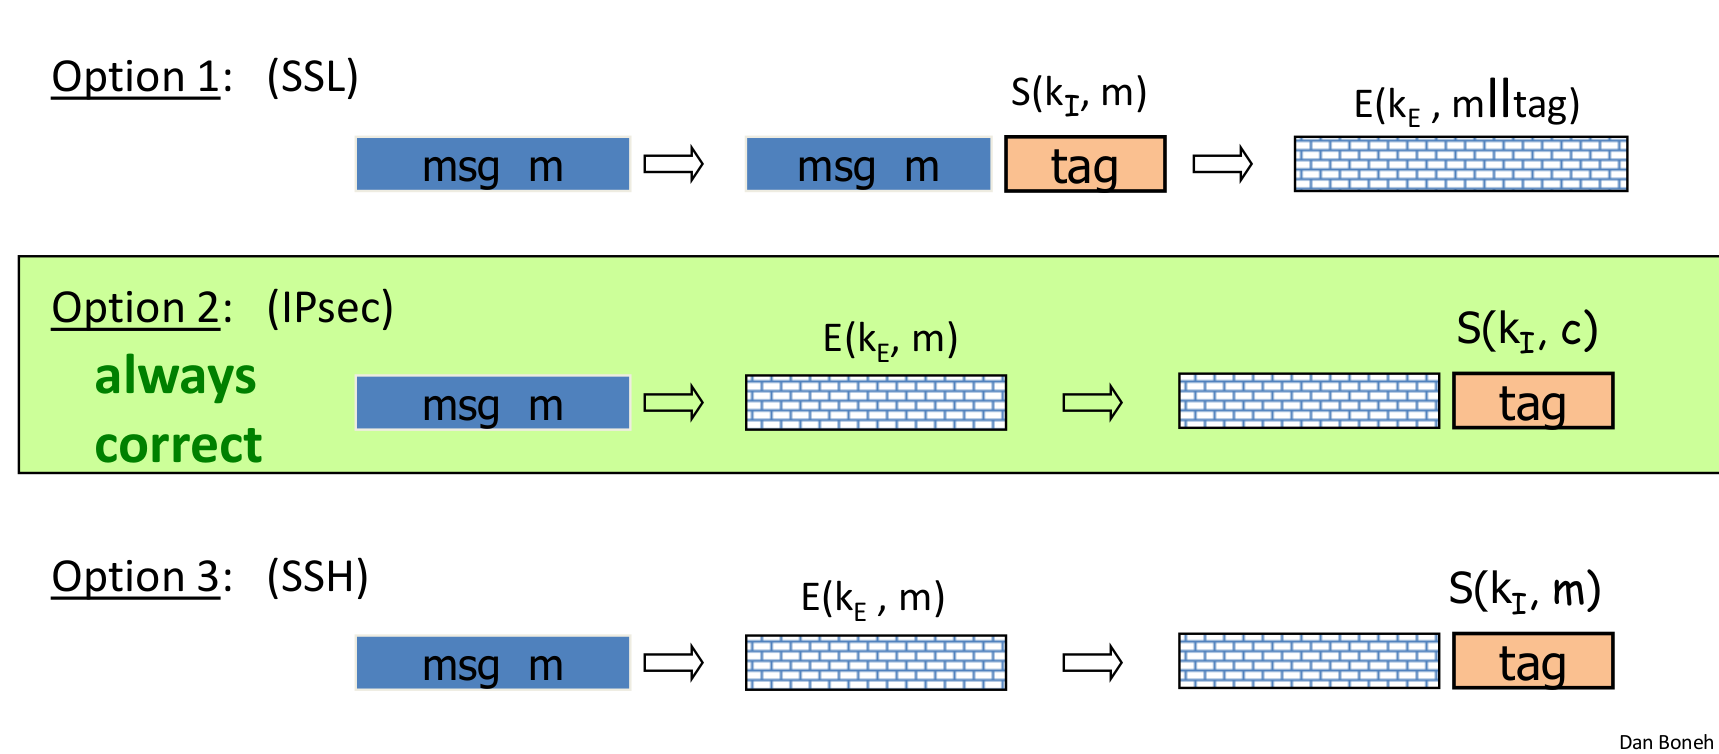
\includegraphics[width=\linewidth]{./img/png/combining_MAC_ENC.png}
\end{frame}

\begin{frame}
  \frametitle{Сочетание шифрования и МАС}

  Пусть ($E$,$D$) -- безопасный симметричный шифр и ($S$,$V$) -- безопасный MAC, тогда:

  \begin{enumerate}
    \item{\textbf{Encrypt-then-MAC} всегда обеспечивает аутентифицированное шифрование}
    \item{\textbf{MAC-then-encrypt} может быть подвержена атакам выбранного шифра}
  \end{enumerate}
\end{frame}

\begin{frame}
  \frametitle{Стандарты}

  \begin{itemize}
    \item{\textbf{GCM} шифрование в режиме счетчика (CTR mode), затем CW-MAC (аппаратная реализация на x86)}
    \item{\textbf{CCM} CBC-MAC, затем шифрование в режиме счетчика (CTR mode)}
    \item{\textbf{EAX} шифрование в режиме счетчика (CTR mode), затем CMAC}
  \end{itemize}
\end{frame}

\begin{frame}
  \frametitle{Стандарт OCB}

  Более эффективный алгоритм (одна операция шифрования на блок)

  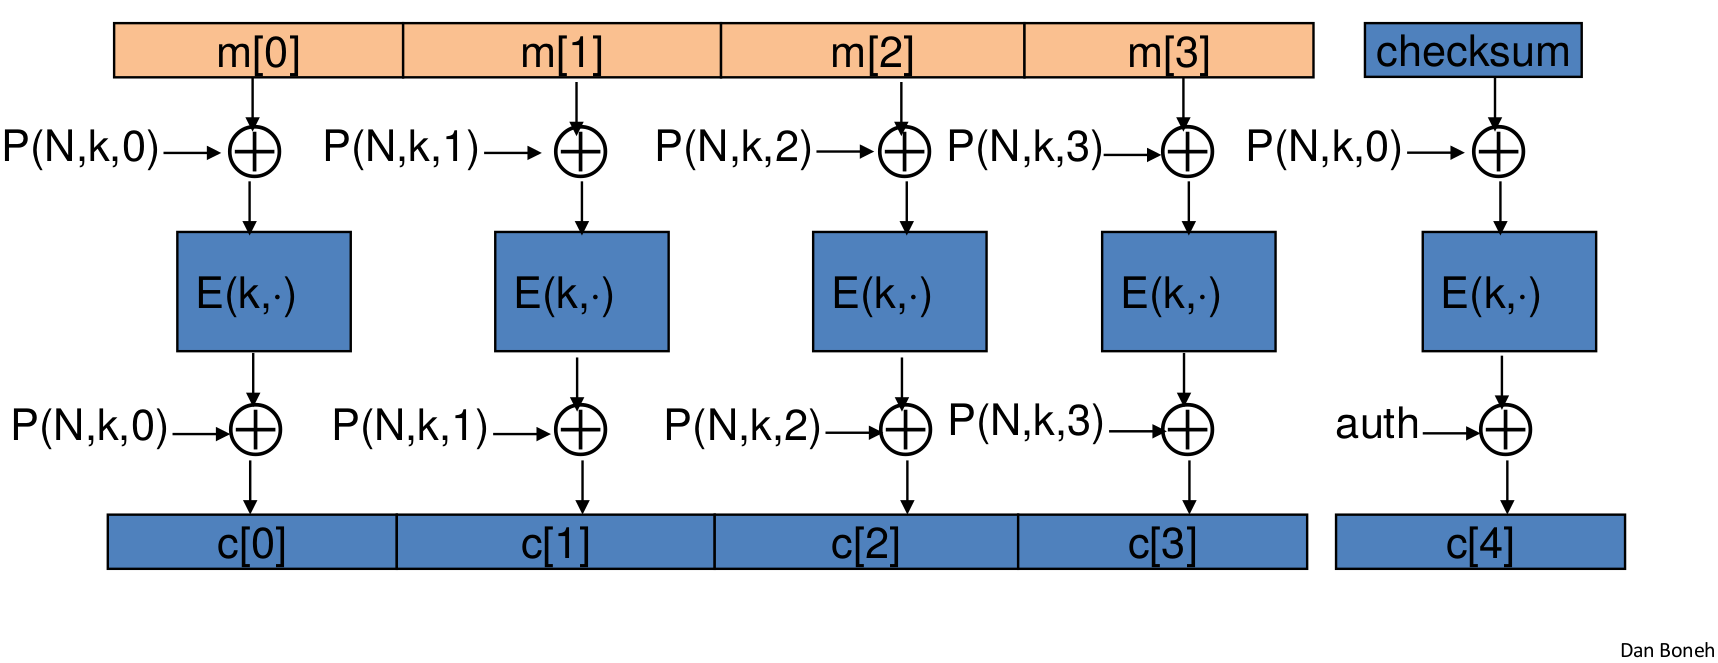
\includegraphics[width=\linewidth]{./img/png/OCB.png}
\end{frame}

\begin{frame}
  \frametitle{Производительность}

  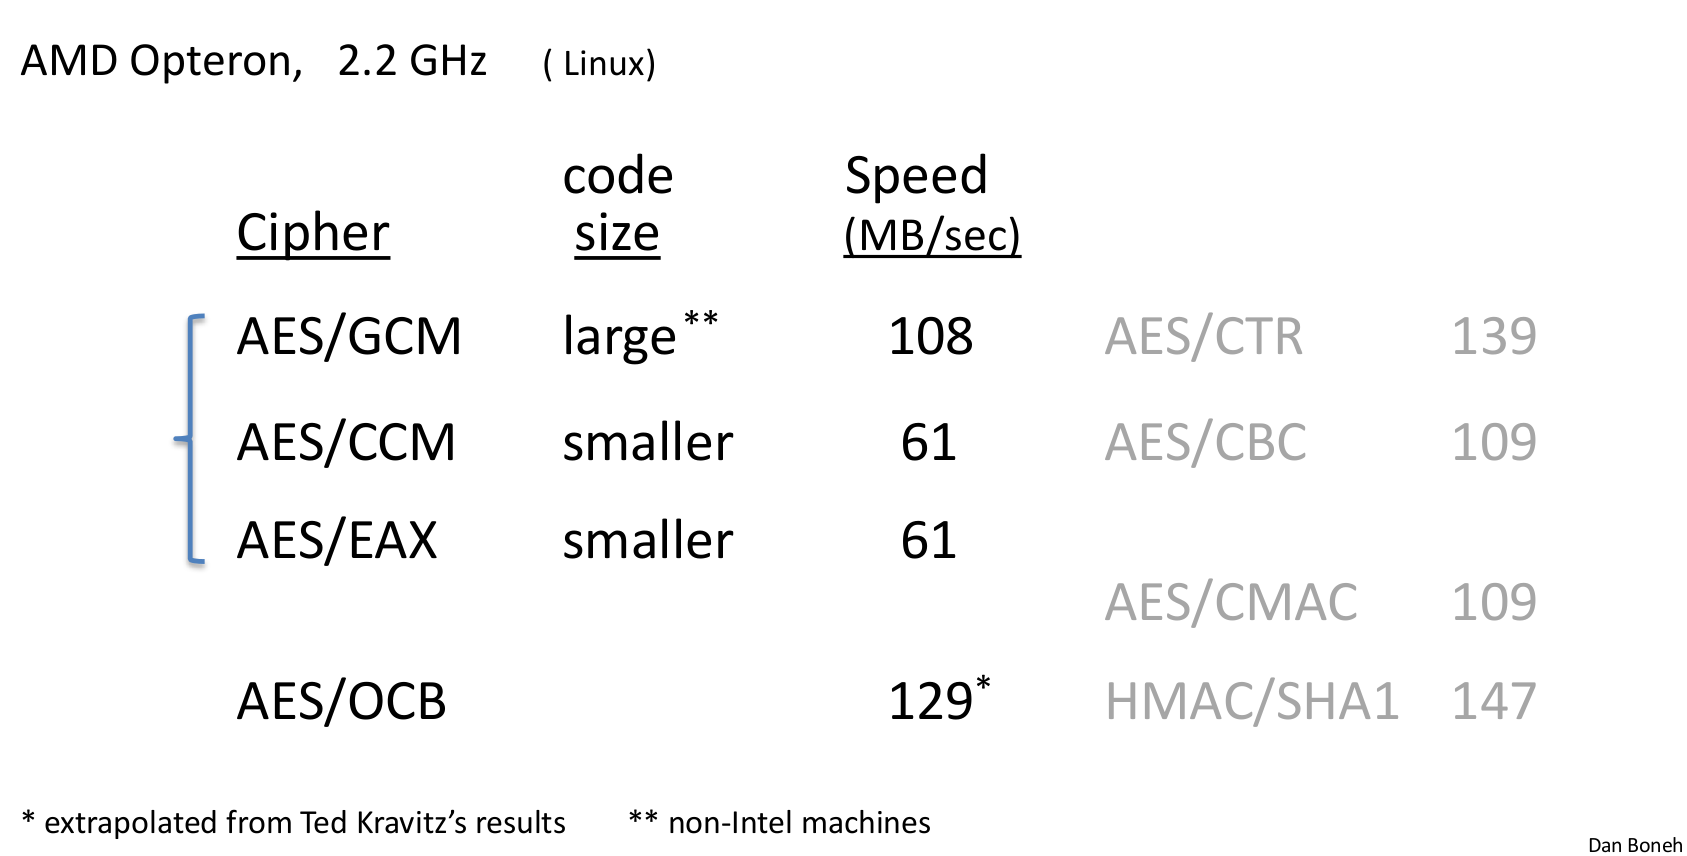
\includegraphics[width=\linewidth]{./img/png/performance.png}
\end{frame}

\begin{frame}
  \frametitle{Пример (TLS)}

  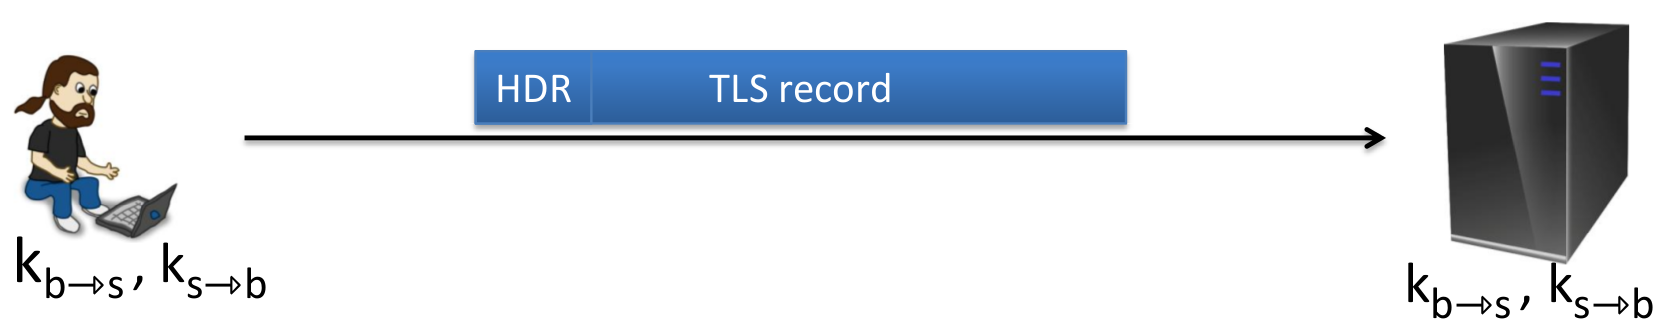
\includegraphics[width=\linewidth]{./img/png/TLS_overview.png}

  Однонаправленные ключи: $k_{b \rightarrow s}, k_{s \rightarrow b}$

  Шифрование с состоянием:
  \begin{itemize}
    \item{Каждая сторона хранит два 64-битных счетчика: $ctr_{b \rightarrow s}, ctr_{s \rightarrow b}$.}
    \item{Счетчики устанавливаются в 0 при старте сессии. $ctr++$ для каждой записи.}
    \item{Назначение счетчиков -- защита от атак воспроизведения (replay attacks).}
  \end{itemize}
\end{frame}

\begin{frame}
  \frametitle{Пример (TLS)}

  Аутентифицированное шифрование (CBC AES-128, HMAC-SHA1)

  $k_{b \rightarrow s} = (k_{mac}, k_{enc})$ 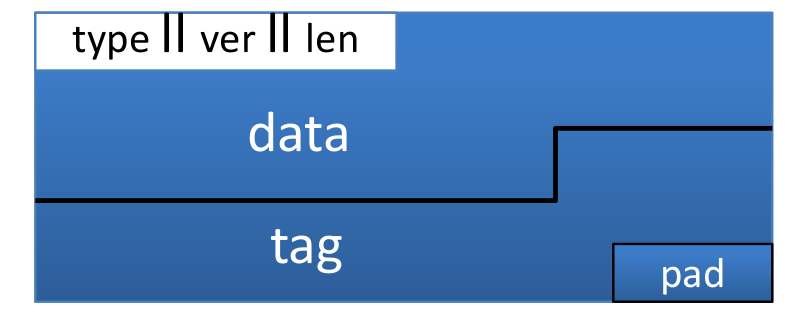
\includegraphics[width=60mm]{./img/png/TLS_record.png}

  \begin{enumerate}
    \item{$ \text{tag} \leftarrow S(k_{mac}, [++\text{ctr}_{b \rightarrow s} || header || data])$}
    \item{Добивка [header || data || tag] до размера блока AES}
    \item{$E_{CBC} (IV, k_{enc}, [header || data || tag])$. IV - случайное }
    \item{Добавление заголовка в начало}
  \end{enumerate}
\end{frame}

\begin{frame}
  \frametitle{Пример (TLS)}

  Дешифрование:

  \begin{enumerate}
    \item{$D_{CBC}(k_{enc},record)$}
    \item{Проверка формата добивки. Ответ \textbf{bad\_record\_mac} в случае ошибки}
    \item{Проверка тега $[++\text{ctr}_{b \rightarrow s} || header || data ]$. Ответ \textbf{bad\_record\_mac} в случае ошибки}
  \end{enumerate}
\end{frame}

\end{document}
